\documentclass{sigchi}

% Use this command to override the default ACM copyright statement (e.g. for preprints). 
% Consult the conference website for the camera-ready copyright statement.
\toappear{}

% Arabic page numbers for submission. 
% Remove this line to eliminate page numbers for the camera ready copy
%\pagenumbering{arabic}


% Load basic packages
\usepackage{balance}  % to better equalize the last page
\usepackage{graphics} % for EPS, load graphicx instead
\usepackage{times}    % comment if you want LaTeX's default font
\usepackage{url}      % llt: nicely formatted URLs
\usepackage{algorithm,algorithmic}

% llt: Define a global style for URLs, rather that the default one
\makeatletter
\def\url@leostyle{%
  \@ifundefined{selectfont}{\def\UrlFont{\sf}}{\def\UrlFont{\small\bf\ttfamily}}}
\makeatother
\urlstyle{leo}


% To make various LaTeX processors do the right thing with page size.
\def\pprw{8.5in}
\def\pprh{11in}
\special{papersize=\pprw,\pprh}
\setlength{\paperwidth}{\pprw}
\setlength{\paperheight}{\pprh}
\setlength{\pdfpagewidth}{\pprw}
\setlength{\pdfpageheight}{\pprh}

% Make sure hyperref comes last of your loaded packages, 
% to give it a fighting chance of not being over-written, 
% since its job is to redefine many LaTeX commands.
\usepackage[pdftex]{hyperref}
\hypersetup{
pdftitle={SIGCHI Conference Proceedings Format},
pdfauthor={LaTeX},
pdfkeywords={SIGCHI, proceedings, archival format},
bookmarksnumbered,
pdfstartview={FitH},
colorlinks,
citecolor=black,
filecolor=black,
linkcolor=black,
urlcolor=black,
breaklinks=true,
}

% create a shortcut to typeset table headings
\newcommand\tabhead[1]{\small\textbf{#1}}

% End of preamble. Here it comes the document.
\begin{document}

\title{One Does Not `Simply' Launch a Citizen Science Project: Reflections on Zooniverse, a Multi-Domain Science Platform}
% \title{A Brief History of Zooniverse: Designing for Multi-Domain Citizen Science}

\numberofauthors{1} \author{ (Authors removed for reviewing) }
\maketitle

\begin{abstract}

\end{abstract}

\keywords{Citizen science, crowdsourcing, interface design}

%% TODO 
\category{H.5.m.}{Information Interfaces and Presentation (e.g. HCI)}{Miscellaneous}

%% TODO 
%% \terms{}

\section{Introduction}

Web-based ``citizen-science'' projects have enabled hundreds of thousands of untrained human volunteers to contribute to open scientific problems across a variety of domains \cite{citizen-science}.  The handful of successful systems have demonstrated that citizen science applications can be valuable both to participants, as educational tools and cognitively-stimulating puzzles\cite{citizen-science-in-curricula}, as well as to scientific researchers who have large unmanageable data sets and problem spaces \cite{fortson-2011, lintott-08, lintott-11, simpson-12, davis-11}.

% zooniverse et al publications >
% https://www.zooniverse.org/publications 
% http://mnras.oxfordjournals.org/content/424/4/2442.full

% davis-12 : The distribution of interplanetary dust between 0.96
% and 1.04 au as inferred from impacts on the STEREO spacecraft
% observed by the heliospheric imagers, Davis+ 2012.  

% sayighs : Repeated call types in short-finned pilot whales,
% Globicephala macrorhynchus, Sayigh+ 2012.

However, designing successful citizen science systems that can be mutually beneficial in this way while sustaining participation over time can be exceedingly difficult.  The reasons are several: first, due to the emerging nature of the field, key design principles and \emph{best practices} are not yet known or established.  The unique aspects of designing for citizen science mean that conventional design methods pioneered for human computation approaches only apply to a limited extent.  For example, human computation systems often apply extrinsic motivation (e.g., direct rewards) to drive participation, while most citizen science participation systems derive from intrinsic motivations of individuals \cite{extrinsic-vs-intrinsic}.  Since such motivations are typically personal and idiosyncratic, designing to drive sustained attention to them is challenging, requiring an understanding of their nature and the activities that inspire them \cite{}.  Moreover, participants naturally engage with citizen science systems in a variety of different ways, and feature a diversity of natural competencies, manifesting in great variation among the ways people interact with the system \cite{raddick}. Finally, the simple fact that, over time, people are likely to simply forget about any particular system, as their attention is turned away towards other, newer systems and activities means that retaining those crucial participants who have accrued a degree of experience and competence in their tasks is significantly challenging.

% we want to switch this from interviews to (in crowd). 
% TODO - Ramine - please update this ``retrospective reflective inductive...''
% to something that makes sense - we sat as a group with key team mebers and identified
% themes

In this paper, we contribute a detailed case-study of a unique citizen-science platform which expanded from a single domain experiment to a ``factory for citizen science'', an authority for generating successful web applications for scientists across domains.  Zooniverse also represents the first system in which volunteer contributions directly resulted in the publication of scientific findings in academic journals, and as of September 2013, has contributed findings to at least $P$ published scientific papers.  The analysis presented here is the result of a retrospective reflective thematic analysis towards identifying key insights and consequences of design decisions gained through the trial-and-error process of generating apps for various domains and data-sets since Galaxy Zoo, the first Zooniverse application.  This iterative process allowed the team to explore design variations at mutiple levels, from the interface/intraction flow, to the design of social elements (discussion forums), to external considerations such as ways to best launch and sustain prolonged engagement through external communications.

% maybe a tad redundant:
The goal of the this paper is to, first, document the informal knowledge gathered by the Zoonvierse team pertaining to how to design successful citizen science projects, based on their experience of launching 24 projects since the platform's genesis.  These insights are then discussed in the greater context of human computation, to derive design recommendations and discuss factors that may be responsible for the observations made. We begin with a short history of the project in order to provide readers a context for the following discussion, followed by a grounded dimensional design analysis of particular aspects of Zooniverse's deployment.  Finally, we discuss Zooniverse's team's perspective of the greatest difficulties for building more effective citizen science: $X$, $Y$ and $Z$, and ways that HCI research may be able to help.

\section{Background: A Brief History of the Zooniverse}

% \emph{TODO: Can someone fill this in?}  The Zooniverse system was conceived .. \cite{fortson2011galaxy} \emph{TODO TODO --- } 

In contrast to crowdsourcing and citizen science projects that focus on participant-driven data collection (e.g., \cite{okolloh2009ushahidi}, \cite{zook2010volunteered}), the focus of Zooniverse is exclusively citizen \emph{data analysis}, that is, having participants help with the classification, labeling and extraction of information from large, already extant datasets. As documented previously by Fortson et al \cite{fortson2011galaxy}, the first Zooniverse project, Galaxy Zoo, was designed to engage volunteers in the morphological classification of images of galaxies, and launched in July 2007\cite{galaxyzoo-launch}.  The first scientific papers that resulted from findings from Galaxy Zoo's over 100,000 citizen contributors were published in 2008, on spin statistics of spiral galaxies\cite{land2008galaxy} and a separate paper on the morphological characteristics of galaxies\cite{lintott2008galaxy}.

After Galaxy Zoo, it became clear to the team that more projects would follow.  The first such was Solar Stormwatch, a project effectively built for the Royal Observatory of Greenwich by Zooniverse.  The first non-astronomy project was debuted in October 2010.

\emph{AND THEN STUFF HAPPENED!} 

%% OUTLINE from Rob >> #TODO turn into a timeline (eMax)
%% After Galaxy Zoo it was clear that more projects were to follow.
%% In develping GZ2 Arfon Smith created `Juggernaut' a Ruby on Rails application, with a MySQL back end, designed as a generalised web application for citizen science projects like Galaxy Zoo.
%% %% Neale this is when the ideas of annotations, classifications etc came into being
%% Early 2010 saw Solar Stormwatch happen, a project effectively built for someone else (Royal Observatory Greenwich) by the Zooniverse. It used Juggernaut and is still running.
%% <<When does the CSA happen!?>>
%% October 2010 sees the deployment of Old Weather - the first non-astronomy project, first transcription project and first to incorporate any game mechanics.
%% Around the same time we began to take social media more seriously and created a blog network, Twitter/Facebook accounts and even held special events such as the (now annual) Zooniverse Advent Calendar in Dec 2010.
%% The Milky Way Project and Planet Hunters launche din Dec 2010 both using public astronomy datasets (like Galaxy Zoo).
%% In July 2011 Anicent Lives launches - another non-astronomy, transcription project.
%% In August 2011 we created `Talk' as a way to begin to better harness the power of our discussion fora. The PHP fora we used beforehand were beocming difficult to support and hard to mine for data. We felt that there was a better user experience to be created and a better way for citizen scienceto happen, base don the experienc eon the Peas Corp and the stor yof the Voorwerp.
%% In August 2011 Ice Hunters went live. Built by a separate development team using our system.
%% In Oct 2011 NEEMO was our first purely experimental project - where we weren't even sure of the scientific outcome. We were very clear about this with the users and even housed it in a new `labs' area of the Zooniverse site to be clear that it was an experiment.
%% Whale FM (Nov 29 2011) was our first project to use sound. It was clear early on that it wasn't as popular as the others.
%% In January 2012, BBC Stargazing Live featured Planet Hunters and we received a million classiciations in just two and a bit days. Planet Hunters was actually more popular in the days following the announcement of our discovering a planet during that time, that it had been during the BBC show.
%% In early 2012 we came up with the idea of switching to MongoDB and HTML5 web-apps served from Amazon S3 buckets. The new system: `Ouroboros' would replace Juggernaut and act as a one app serving all our projects. The Juggernaut codebased had become fragmented and each project required its own server and DB. It was getting expensive! IN Sep 2012 we ran `Citizen Science September' and launch four projects in four weeks. These were all base don the new system and it worked out very well.
%% BBC Stargazing returned and in Jan 2013 we launched Planet Four, built specially for the show.
%% AT writing, the latest project was Worm Watch Labs, the 27th project launched in June 2013.

Table \ref{project-summary} lists all of the Zooniverse projects,
launch dates, sizes of data sets and classifications as of September
2013.  Figure $Y$, likewise, illustrates the growth of the project
from June 2007 until September 2013.

The complete list of scientific papers that have resulted from
Zooniverse are compiled on the Zooniverse web site\footnote{Zooniverse
  Publications - \url{https://www.zooniverse.org/publications}}.

% Terminology of Zooniverse 
% See blog post by arfon > 
% The Zooniverse team have developed a shared vocabulary for discussion
% of the system, which resulted from knowledge gained throughout $5$
% years of project building as well as patterns resulting from working
% with science teams.

% \emph{Users} are the volunteers using the system. Each user entity
% consists of a username, email address, information about the projects
% they've used and other related pieces of information.

% \emph{Subjects} are the individual assets which users are shown when
% classifying. They may consist of images, audio files or videos.

% \emph{Tasks} are the activities which users carry out when presented
% with a subject.

% \emph{Workflows} are groups of tasks.

% \emph{Classifications} are made up of the user, subject and task
% entities.

% \emph{Groups} are groups of subjects - Subjects from a particular
% time period or 'season' in the Snapshot Serengeti project  may form 
% a group, for example.

% \emph{Projects} are overarching entities with which subjects, groups
% and classifications are associated. In the Ouroboros API used by 
% Zooniverse, project entities store information about groups and the
% status of the project, as well as other administrator functions.


\begin{table*}
\begin{center}
\caption{Summary of Zooniverse projects past and present.
Notes: The 1.68 million assets in the various Galaxy Zoo projects are not unique, since galaxies in GZ1 were used in subsequent projects.}
\begin{tabular}{lcllclll}
\hline
Project & Status & URL & Launch & Category & Logged-In & Assets & Interface \\
Name &  &  & Date &  & Users &  &  Type \\
\hline
\hline
Galaxy Zoo & Retired & zoo1.galaxyzoo.org & 11 Jul 2007 & Space & 165,000 & 890,000 & Classification \\
\hline
Galaxy Zoo 2 & Retired & zoo2.galaxyzoo.org & ?? ??? 2009 & Space & XX,XXX & 304.122 & Classification \\
Galaxy Zoo Mergers & Retired & mergers.galaxyzoo.org & 23 Nov 2009 & Space & 20,588 & 58,956 & Classification \\
\hline
Solar Stormwatch & Active & solarstormwatch.com & 22 Feb 2010 & Space & 65,971 & YY,YYY & Classification/Marking \\
Galaxy Zoo Supernova & Retired & supernova.galaxyzoo.org & 26 Mar 2010 & Space & 37,150 & 76,376 & Classification \\
Galaxy Zoo: Hubble & Retired & zoo3.galaxyzoo.org & 17 Apr 2010 & Space & XX,XXX & ~200,000 & Classification \\
Moon Zoo & Active & moonzoo.org & 11 May 2010 & Space & 121,251 & 435,314 & Marking \\
Old Weather & Active & oldweather.org & 12 Oct 2010 & Climate & 32,076 & YY,YYY & Transcription \\
The Milkyway Project & Active & milkywayproject.org & 07 Dec 2010 & Space & 57,675 & 35,695 & Marking \\
Planet Hunters & Active & planethunters.org & 16 Dec 2010 & Space & 167,354 & 3,063,759 & Type \\
\hline
Ancient Lives & Active & ancientlives.org & 25 Jul 2011 & Humanities & 24,983 & 153,885 & Transcription \\
Ice Hunters & Retired & icehunters.org & 09 Aug 2011 & Space & 15,276 & YY,YYY & Classification/Marking \\
NEEMO & Active & neemo.zooniverse.org & 15 Oct 2011 & Space & X,XXX & YY,YYY & Classification \\
Whale FM & Active & whale.fm & 29 Nov 2011 & Nature & 2,150 & 15,531 & Classification \\
\hline
SETI Live & Active & setilive.org & 29 Feb 2012 & Space & 63,609 & YY,YYY & Type \\
Galaxy Zoo 4 & Active & galaxyzoo.org & 11 Sep 2012 & Space & 48,550 & 390,907 & Classification \\
Seafloor Explorer & Active & seafloorexplorer.org & 13 Sep 2012 & Nature & 14,099 & 123,077 & Marking \\
Cyclone Center & Active & cyclonecenter.org & 27 Sep 2012 & Climate & 4,767 & 196,638 & Classification \\
Bat Detective & Active & batdetective.org & 02 Oct 2012 & Nature & 1,580 & 582,203 & Classification \\
Cell Slider & Active & cellslider.net & 23 Oct 2012 & Biology & 13,261 & 275,702 & Classification \\
Andromeda Project & Active & andromedaproject.org & 05 Dec 2012 & Space & 5,072 & 12,425 & Marking \\
Snapshot Serengeti & Active & snapshotserengeti.org & 11 Dec 2012 & Nature & 22,173 & 1,240,727 & Classification \\
\hline
Planet Four & Active & planetfour.org & 08 Jan 2013 & Space & 34,718 & 98,920 & Marking \\
Notes from Nature & Active & notesfromnature.org & 22 Apr 2013 & Nature & 3,490 & 123,402 & Marking/Transcription \\
Space Warps & Active & spacewarps.org & 08 May 2013 & Space & 9,544 & 345,240 & Marking \\
Worm Watch Lab & Active & wormwatchlab.org & 30 Jun 2013 & Biology & 3,251 & 74,016 & Classification \\
\hline
\end{tabular}
\end{center}
\label{project-summary}
\end{table*}



% TODO (from Chris): Guide to the Social Science papers that have been written
% TODO add a guide to the Papers that contain project descriptions for each project

\section{Method}
\emph{TO BE WRITTEN LATER}
%% Four sessions were dedicate to performing a group thematic
%% analysis. Participants from the Zooniverse team included the team
%% lead, lead project manager, and two designers of the Planet Hunters
%% application.  Interviews were recorded and transcribed,

%% inductive process which led to the themes for the coding analysis.
%% These themes were used as the basis of a second round of interviews
%% focused on these themes, upon which a second coding process was
%% applied by 3 researchers

\section{Dimensions for Design}
% Themes? Observations?

\subsection{Key components of a citizen science project}

Despite the development of projects in very different domains of academic research, and which involve disparate user interactions, the core requirements for a successful citizen science project remain stable. A `main' interface allows a \emph{user} to complete a \emph{task} when presented with a \emph{subject}. The task is typically constrained by the tools provided (e.g. answer questions from a decision tree, mark craters on an image) and when completed typically results in the presentation of the next subject to be classified. In Zooniverse projects to date, participants perform tasks individually, and are typically not given control over choice of what subjects to work on. This latter choice makes deliberate manipulation of the data difficult and also ensures that project priorities are respected (i.e. it's not just the beautiful/interesting/easy subjects that are worked on). Secondly, some tutorial elements - either as a stand-alone tutorial, as an interactive within the interface or as surrounding context - are required to acquaint users with their tasks. An additional environment for discussion is typically, but not always, provided allowing for more free-form interaction between users and other participants such as scientists, developers and for which work goes beyond the initial task. Extra tools for manipulated subjects or for exploring contextual information may be provided in association with these discussion environments. 

A community of participants is implicitly necessary for a citizen science project; crowdsourcing without a crowd is a perhaps unsolvable problem. However, levels of participation and involvement in the community will naturally vary; Zooniverse projects typically receive a substantial number of their classifications from users who will never return. A successful citizen science project will thus be designed to both enable these short-term participants to make useful contributions while still fostering longer-term engagement. This need also illustrates the requirement in most cases to assess the ability or accuracy of participants; many projects thus incorporate `tests', either explicitly or more commonly by including simulated or expert-classified subjects in the workflow presented to users. 

\subsection{Discussion forums}

% ``number of emails received by the team'' -> what kind of emails? and how did this prompt use of a forum
%% Michael Nielsen's book > on networked science --- Reinventing discovery
%% http://press.princeton.edu/titles/9517.html

The original Zooniverse project, \emph{Galaxy Zoo 1}, launched as a standalone site without a discussion environment, but a forum was added soon after launch\footnote{The original forum is still active at \url{www.galaxyzooforum.org}}, primarily in response to the number of emails received by the team. The forum unexpectedly became a vital part of the scientific machinery supported by Galaxy Zoo, with users making use of the site to identify, discuss and advocate for serendipitous discoveries. The canonical example is the object now known as Hanny's Voorwerp \cite{voorwerp}, a galaxy-scale glowing gas cloud which turned out to have been ionized by activity associated with neighboring galaxy's rapidly feeding black hole. In this case the discovery was reported on the forum, but the follow-up work was carried out by the science team themselves. In other examples, though, much more sophisticated behaviour was seen. The discovery of the Galaxy Zoo Peas \cite{Peas}, for example, saw a group of volunteers who had identified the presence of small, round and green objects (hence the name) in the background of some images work together to download and explore metadata on these objects, to write database queries and even, eventually, to create their own citizen science site to assist in further classification of these intriguing objects. The peas turned out to be a new class of galaxy, the most efficient stellar factories in the local Universe, and remain the subject of vigorous debate in the professional astronomical community. 

Structured collaboration also proved effective. Galaxy Zoo science team member Bill Keel from the University of Alabama was able to spend time on the forum, and asked for help with searches for objects such as galaxies which appear to overlap \cite{overlap} (distant galaxies used to illuminate foreground ones can be used to probe the dust content of systems, a matter of some importance to astronomers). This work was also successful, but required Keel to spend substantial time as part of the forum community, something that other science team members were unwilling or unable to do. Furthermore, by 2009 the forum had become less popular; the percentage of Galaxy Zoo users posting on what was a standard \emph{Simple Machines forum}\footnote{} was very low (less than two percent) and with more than 500,000 posts in more than 10,000 topics it had become difficult to navigate. While it still served the need of a core constituency, it was not engaging the majority of Galaxy Zoo classifiers in science. The low participation rates were mirrored in other Zooniverse projects such as Moon Zoo and Old Weather, although the latter in particular provided a core community with a space to discuss the historical aspects of the project in particular.

Starting from the launch of Planet Hunters in 2010, Zooniverse projects have made use of a custom discussion environment known as `Talk'. It was designed to enable links to be made easily between classification and discussion and to allow science team members as well as advanced volunteers to quickly notice when users were talking about discoveries of potential interest. To understand the design drivers for talk's system of object-orientated discussion, consider the case of a new classifier who had spotted a `pea' in a Galaxy Zoo image. Even if they were to move to the forum, they would have been unable to search for discussion of their or similar objects unless they made the same mental leap to think of a small round celestial object as a kind of vegetable. If they found the right thread, they would have had to upload their image to a linear discussion which might well be in the middle of more detailed analysis. In Talk, by contrast, a single click after classification invites discussion, and lands on a page dedicated to discussing the object that's just been classified. Our putative pea-finder would immediately be able to see what had already been said about this system, and - were it already to be tagged as a 'pea' - to click on 'pea' and realize that there was a much broader conversation going on. This model has been broadly successful, with most of the discoveries made by the Planet Hunters project (including PH1b, the first planet in a system with four stars) coming from discussion between users who found interesting things in the interface and a community of more advanced workers who were able to help the science team follow-up on those discoveries. 

Participation in Talk is triggered in different ways for different projects. In Planet Hunters the question 'Would you like to discuss this?' is asked after each subject is inspected, increasing engagement with Talk at the cost of slowing down classification in the main interface. As much of the Planet Hunters science has come from Talk, this trade seems worth making. In fact, the main interface is serving two important functions - it is both providing classifications as designed, but it is also providing entry points to discussion. In particular, this second function produces science through the intervention of `superusers' who may not classify themselves but who are able to make use of and further analyze interesting discoveries. 

In the Milky Way Project, launched a few weeks later, Talk is offered as one as three options after work on a particular subject is completed ('Save', 'Save and Discuss' - which leads to Talk, and Cancel). We might predict that the Milky Way Project Talk will be less popular, and indeed it is (XXX DATA? XXX). However, another significant factor influencing the success across instances of Talk seems to be involvement of the science team in discussions, especially in the first few days of a project. Early engagement allows trust to build up between moderators, community and professional scientists which sustains a community in the long term. This is now a key consideration in project selection and timing of launch. 

Citizen scientists who wish to contribute to the community in ways beyond simple classification have found other ways to do so. For example, Zooniverse discussion spaces are moderated not by the science team, but by volunteers, typically chosen from amongst those who participate in the beta test. Volunteer moderators have set community standards, produced substantial texts and guides for new participants and often act as a liaison between volunteers and science team, and it seems advantageous to distinguish between those providing expertise (typically the science team) within a community and those responsible for shaping and policing it. More recent projects have involved moderators and advanced users in the process of development; the Andromeda project includes Jules Wilkinson (moderator on Moon Zoo and Solar Stormwatch) as a full member of the project team, and Space Warps included XXXX of their likely volunteers in their initial workshop where the concept for the project was developed. 

Different prompts to talk.
Discussion of talk features. 

Galaxy Zoo Peas Corp and Hanny's Voorwerp.
Created Talk and then found cool planets in PH, Yellowballs tag in MWP, Convict Worm in Seafloor

% \subsection{Forums}
%% Forums -> 
%% Introduction of Talk 1.0 -> 
%% Introduction of Talk 2.0
%% Organisation and Fragmentation 
%% Top level organisation, moderators, scientists and how this has changed and impacted 

%% In a study investigating the effect of instructors on forum participation, Mazzolini and Maddison found that instructors who posted frequently on a forum on average produced shorter discussion threads \cite{mazzolini2003sage}. In the Zooniverse environment the participation of `moderators' and `scientists' could be hindering the discussion flow between general science citizens. Furthermore there was a negative correlation between instructor initiated conversations and participation, especially in the advanced units\cite{mazzolini2003sage}. 

%% @Neal does this support your findings so far?
%% Conversations started by moderators tend to be ignored
%% except in the case of particularly 'controversial' posts,
%% such as threads about the I don't know button. However,
%% such threads tend to be FAQ-style single post Q&A threads,
%% and so it's possible this is why. In fact 'welcome' style
%% threads are almost always started by moderators and these
%% threads are among the most popular threads across all projects.
%% However, certainly where moderators attempt to engage in
%% pre-existing discussion threads, their comments are ignored and
%% their questions go unanswered, except usually, by other
%% moderators, although this may partially be a result of the
%% subject matter or the time which has elapsed (necromancy). 

%% In terms of frequent posters, that's something I'll look into

%% Success stories: examples of super-moderators who externally test
%% contributions and distill them for the scientists
%% (why only in certain apps and not others?)
%% (how do super moderators affect the community // roles played)
%% Space Warps - Moderators and users teaching other users to use
%% modelling software to model subjects, in order to help
%% identify lenses. Seemingly entirely voluntarily, as posts point
%% out how unexpected these contributions were at this stage

\subsection{Tutorial}

As noted above, a tutorial experience is an essential part of a citizen science project, but designing a tutorial brings one into conflict with several other requirements. In particular, Zooniverse projects are designed to get useful classifications from those who only visit once; an overly elaborate or time consuming tutorial leads to these casual visitors leaving without ever having done anything `real'. This is problematic not only in terms of lost effort but also in failing to present an authentic experience of participation, the very thing that seems to engage potential citizen scientists to return. Tutorial design, therefore, has tended to emphasize presenting only the 

The original Galaxy Zoo included only a few lines of tutorial, followed by a simple test (as described in \cite{Lintott}). The aim of this was both to ensure a minimum level of classification accuracy and to provide feedback to users who it was felt might need reassurance that they were on the right track. However, to encourage participation the bar was set extremely low and the test was essentially ineffective; classification accuracy was ensured by later data reduction, a pattern followed by subsequent projects. Galaxy Zoo 2 included a longer, optional, tutorial which few users read, leading to the adoption (by, for example, Moon Zoo) of video tutorials which no-one watched. The solution now adopted was an inline tutorial which guides users through the interface quickly and gives feedback on classification of one or more initial subjects.

This solves the problem of teaching classifiers what is expected of them, but consistent learning takes place throughout a citizen scientists' career. \cite{Smith}, for example, show trajectories of classification accuracy for individual users, showing that while large changes most often come early in a user's encounter with a project dramatic changes in accuracy are possible throughout. Each classification provided by a user produces a (perhaps unknown) change in user behaviour through learning, information about the subject under classification and information about the user themselves. Projects such as Planet Hunters, the Andromeda Project and Space Warps include expert-classified or synthetic data which can be used to measure user performance. When presented with synthetic data feedback is given to the user on their performance - essential in preventing them getting excited about discovering simulated planets but which also forms as an ongoing tutorial. 

Video tutorials don't work. People do them but then leave (SSW).
Compulsory training results in a large bounce rate (Moon Zoo)
With Whale FM and Ancient Lives we used tutorials that were interactive and overlaid on the interface - seemed to work well.
Then we moved on to the next logical step, which is guiding a user through a classification by annotating the interface as they go along. That's where we are now.

% when we turned on compulsory tutorial -- bounce rate went up

\subsection{Interface Design}

% Does good design improve participation?  Much evidence has suggested that \emph{good design builds trust}, by improving people's subjective appraisal of web sites and applications.  

%% Examples of surface level/aesthetic re-design >  (and perceived effects)
Moon Zoo : redesigned December 2011 - re-designed the web site around the interface, interface had a slight modifications, and perceived effect? % look to see if there was any effect? >> not as far as we can see

%% Examples of thematic redesign encompassing addition of narrative context (and percevied effect) > 
How to measure engagement
  how much time spent on the site
  people stick over a minute, (2-3 mins, high is 20)
  (moderators of old weather)?
  % TODO: can we say anything about the effect of the narrative in Old Weather? 
  % evidence in the discussion forums ? 
  %   > i wonder why the handwriting has changed?
  %   > most keen to help each other out -- 

%% Examples of interface affordance design (and perceived effect)
GZ / GZ2 - so it was turned into a deicsion tree
  what kind of galaxy, 6 buttons -> decision tree
% much better data, and it decreased participation

% I DONT KNOW button - don't have one (blog post)

% Surface design doesn't matter

Good design builds trust. There is implicit trust in a website that matches the expectations of web users. Online interfaces are judged (consciously or otherwise) in comparison to the pages that a user has recently visited (often only seconds previously) and pages they regular visit. A rising tide of improving visual aesthetic has resulted from a decade-long virtuous cycle of modern websites attempting to keep pace with the standards of more sophisticated users, which in turn has raised users' expectations.

A well-designed website creates trust in new users and comfort in returning visitors. It also encourages sharing by others.

The trajectory of design at the Zooniverse changed dramatically in 2010 with Old Weather, the Milky Way Project and Planet Hunters. % 

Ice Hunters is the exception: a project widely derided for its design, that was very popular and encouraged people to make thousands of classifcations. Could this be an indication that ease of use and accessibility (the goal of Ice Hunters wa sclear and easy to understand) trumps design, at least in the short term.

In 2012 and 2013 there has been a rising fraction of users accessing Zoonivers sites via an iPad. This has led us to test more on iPads, but not to ensure total compatibility. Rather those projects which are suitable for table use -- meaning those that would not be hindered by users operating the site with their fingers on a smaller screem -- are tested for functionality on tablets in general.

\subsection{Launching Projects}
% Andromeda, Whale FM, Spacewarps and Snapshot Serengeti as case studies

With more than 20 projects launched over just a few years, the Zooniverse platform is host to a series of natural experiments regarding the announcement and subsequent take-up of citizen science projects. There are a large number of variables affecting the potential uptake of any new site including but not limited to; method of announcement (e.g level of press coverage, size of exisiting community), `stickiness' of proposition (i.e. discovering an exoplanet is generally more exciting as a proposition than differentiating genetic subsamples of nematode worms); difficulty of task; technological requirements (e.g. Does the site work on desktops, tablets, smartphones); and many more.

\begin{figure}
\centering
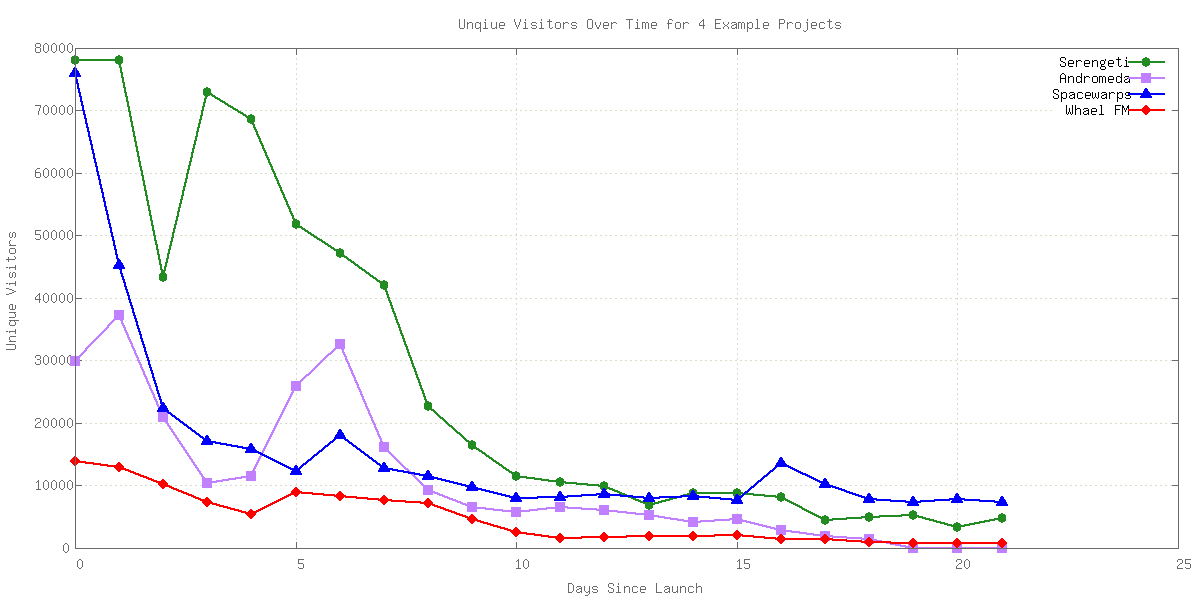
\includegraphics[width=0.48\textwidth]{data/launch-profiles/launch-profiles.png}
\caption{Launch profiles for 4 example Zooniverse projects.}
\end{figure}

Shown above are the first three weeks of activity on four Zooniverse projects: Whale FM (Nov 2011), The Andromeda Project (Dec 2012), Snapshot Serengeti (Dec 2012) and Spacewarps (May 2013). Each project displays a subtly different profile of activity in its first days and weeks.

%Add annotations to this plot and talk about events that influenced the profiles. Note that the launch iof Serengeti gives Andromed a boost a week in.
\subsubsection{Response from Exisiting Zooniverse Community}

After the launch of every project the whole Zooniverse community is emailed an announcement with an explanaiton of the project and how to take part. This pre-exisiting set of users -- who already have a sign-in for any new zooniverse site -- is often enough to create a sizeable surge in activity in rhe arly days of a project. In cases where no press coverage exists this initial boost is sometimes cruical in producing useful data. The case of the Andromeda Project is particularly interesting. This was the Zooniverse's first new space-based project for almost a year and it did not receive signfiicant press coverage. However the resposne from the Zooniverse community was so large that it completed it's entire requirement of 1.1 million classification in just over two weeks. Similarly, the initial surge in traffoc on the Spacewarps project was impressive (10,000 people contributed 500,000 classifications in 24 hours) and sustained (more than 10,000 people were visiting the site every day even three weeks later), and it took days for blogs and news sites to pick up the project and publish about it more widely.

\subsection{Sustaining Engagement}

From the very first moment that a user arrives on a website, they are more likely to leave than to stay. The faster they can be engaged with participation in the main (citizen science) task, the more people will have participated over all.

A `Call to Action' appears to work increbily well. Sites with clear, succinct front-page descritpions ot a project's intention have lower bounce rates over all (the fraction of people who leave and don't classify). This was first seen clearly with Planet Hunters but also with Galaxy Zoo's fourth incarnation.

Projects with innately simple tasks (e.g. Ice Hunters, Spacewarps) show much higher classifications-per-user numbers than projects with more complex tasks (e.g. Milky Way Project, Cyclone Center). The complexity of a task does not appear to be correalted with how long users spend on the site in any session. Moon Zoo and the Milky Way Project have similar interfaces but very different dwell times. Conversley, Ice Hunters and Old Weather had similar dwell times for many months, despite one being far more complex than the other.

\subsubsection{Speed/Latency}

Creating a responsive online environment requires more sophicasted back end technology. Classification subjects must be drawn out of the whole set on a per-user basis (e.g. users should not see the same subject twice). This creates load on the database every time a new user comes to the classification interface. This situation creates a problem with large datasets, where grabbing a random subject could take up to several seconds; a very long time on a website. The need for reduced load times led to the adoption of \emph{Redis} a database/queue system that can deliver random assets quickly. It also prompted a move away from standard \emph{MySQL} databases per-project and toward a unified \emph{MongoDB} datastore.

The combination of \emph{MongoDB} and \emph{Redis} means not-only faster websites, but also allows for more complex subject selection rules. For example, it becomes possible to group-up and prioritise subjects, or vary the numbe rof required classifers over time. Significantly it hasd allowed for subjects to be retired from classification if they contain nothing ot note. This has hugely improved the issue of projects with intrinsically less-appealing or repetetive datasets.  

\subsubsection{Interaction During Classification}

In addition to the above section on tutorials, there are other ways to give users feedback about their efforts in citizen science.

Since Galaxy Zoo 2 there have been occaisional project-`ometers' created to show progress of the community toward a common goal or project completion. The Planet Hunters `Planetometer' displays the total number of classifications of the project, as well as the number planet candidates discovered. The `Moonometer' shows the cumulative area of the Moon that Moon Zoo has scoured for craters in various units\footnote{Units include Square Miles, Football Fields, Taj Mahals, Switzerlands, Utahs, Texas, Polands, Wales, Whales and others -- see http://www.moonzoo.org/moonometer}. These counters exist on many projects but not all.

Where they do exist these counters do not normally appear to drive people to participate, but they do appear to be heavily discussed by people writing about projects and by dedicated users noticing the approach of milestones. In the case of Galaxy Zoo 2 there was a drive toward 60 million classifications in March 2010, to mark the completion of the project; whereas in Old Weather the imminent arrival of `100\% Complete' on the homepage caused users to slowdown and literally ration themsevles to abait the project's conclusion.

Individual counters of a single user's classifications have existed for several projects as well as result in people talking about their own classification count. A volunteer's counter for all projects has existed on the the Zooniverse homepage\footnate{http://www.zooniverse.org} for two years but is rarely discussed and in fact many regular users of the site have no idea it is there!

More recent Zooniverse projects have been able to include synthetic or expert data. This has meant that in many cases a user can be given instant feedback on their classification. The reaction to has been almost universally positive, and it appears to give confidence to some users who might otherwise have not continued with the project. The most recent example is Sapcewarps, which gives continous feedback, although at an ever-decreasing rate, throughout a users time on the site.

\subsubsection{Social Media}
% favouriting, tweeting, blog posts
Often the majority of posts in an online forum are contributed by a minority of active participants, also referred to as the "power law distribution of participation" \cite{lampe2010motivations}. 

\section{Discussion}

\subsection{Common Myths of Citizen Science}
\subsection{$D$ Myths of Designing for Citizen-Science}
\subsection{Myth $X$: Putting new users through a `tutorial is a good idea}
\subsection{Myth $Y$: Citizen science projects have to be `gameified'}
%% to gameify or not?
McGonigal identified four defining elements of a game: a goal, rules, feedback system and voluntary participation. Other features such as leader boards, badges, the `winning' sensation are all used to reinforce these core concepts but do not create a game environment in their own right \cite{mcgonigal2011reality}. To further this gameplay is a state which encourages an optimistic outlook on personal capabilities, partnered with `invigorating rush of activity' \cite{mcgonigal2011reality}. These concepts would support a science citizen, creating a gameplay state to highly motivate and encourage them to undertake difficult challenges. 
\subsection{Myth $Z$: Participants become domain experts}
\subsection{Myth $Z$: Images don't have to be beautiful and graphs don't have to be scary)}
\subsection{Myth $Z$: If You Build It, They Will Come}

It is a common misconception that websites are busy by default. It should go without saying that publicity and attention are required for people to find an online citizen science project. Networks and communities exist online to allow people to discover and share online projects. The Zooniverse was one of the first organisations in this field and has grown a substantial network of people around it (\~860,000 at time of writing).

However above simple awareness, any creator of a citizen science project should be awrae of the approximate effort required. Most Zooniverse sites enlist the help of tens of thousands online volunteers. Thus when projects are designed, consideration should be given to the scale of the endeavour being attempted. Taking into account a reasonable expectation of wbe traffic and the effort any person may put is is difficult (how long is a piece of string?) but improtant for establishing a project with a realsitic end goal within the required time. Simply producing a citizen science website does not guarantee popularlity -- or more importantly scientific completion of the indended task.

\subsection{Myth $Z$: Moderator involvement encourages discussion}
Studies conducted in the educational sector have discovered that contrary to popular belief, instructors (i.e. experts) who contribute often to discussions actually decreased student posts \cite{zydney2012creating}. However, Mazzlini and Maddison propose that this reduction could be a result of more efficient discussion and understanding \cite{mazzolini2007jump}. 

In a forum context, an interactive post is one which responds or replies to another's message, whereas a participation is the number or length of a post \cite{schrire2006knowledge}. 
Schrire discovered two distinctive interaction patterns: instructor-centered, messages predominantly responded to the post by the instructor and synergistic, student-student collaboration \cite{schrire2006knowledge}. 

\subsection{Themes We See Support For}
\subsection{Design Builds Trust}
\subsection{Scaling/latency and practical deployment constraints during design}
\subsection{What makes a good citizen science project?}

\subsection{Comparison to Other Systems}
% Comparison with Jeremy Bentham project - failed in the sense that required more energy than was gained out of it, 20 people at the end
% YourPaintings
% Be A Martian

% \subsection{A Heuristic Framework for Citizen Science App Designers}

%% In order to put the observations described above into a more concise, easily communicated and form, we assembled common themes into a multidimensional framework of design heuristics for citizen science system designers, comprising 6 constructs, described below.  Each construct is meant to address a key dimension of the necessary components described earlier, using the observations discussed in findings. The purpose of such a framework is intended both as an artefact for discussion and refinement, and potential practical use by designers seeking to apply insights from the Zooniverse team  currently made by the Zooniverse team.

% attracting new users' attention / expanding the user base
% identifying 'good' projects - understanding what can be turned into a good Citizen Science project
% contextualising the project
%   interestingness/difficulty/conceptual+contextual+narrative threads that tie the tasks together
%
% performing the task - 
%   - tutorials
%   - elicitation/task vtrtvgtvvt4interface considerations // wide open, specific labeling, decision trees
%   - levels of design and their considerations (aesthetics, challenge, interestingness)
% discussion and collaboration - 
% retaining experienced + most valuable participants
% dealing with new data ~
% distilling knowledge from contributions : (amalgamating responses into thing)


% other/misc
%   transferring interest to other projects
% almost always needs a discussion space

\subsection{Engagement: Interestingness x Difficulty x Context}


% \subsection{Unsolved mysteries}

\section{Related work}

% anyone elses' citizen science systems
\emph{Connect related work here with FoldIt, etc}

\section{Conclusion}

\section{Acknowledgments}
Acknowledgments omitted for blind review.

\balance

%% The Zooniverse framework team has derived significant has
%% been successively refined and scaled as the variety of tasks and
%% number of participants have increased.  At its current state,
%% currently having launched $X$ distinct applications for $Y$ scientific
%% domains, including astronomy, zoology, cell and marine biology,
%% archaeology and paleontology.  This platform represents a unique\cite{moore2011facebooking}


%%  These
%% applications, though separate, have been built on top 

%% The experiences from the first were used to derive design goals for
%% the next,

%% The contributions of the 
%% We identify key design challenges

%% especially as the best practices for designing citizen science systems
%% has not yet emerged.  Among the many design challenges include, being
%% able to appeal to participants with an extremely wide range of
%% expertise, ranging from no knowledge of the field to significant
%% background and interest.  Participants naturally feature a diversity
%% of natural competencies, which is manifested in some people being
%% simply much more adept at some tasks than others. Second, people have
%% many different reasons for engaging with citizen science projects, and
%% to sustain engagement, these platforms must appeal to, and engage
%% these different motivating reasons. Finally, there are a large variety
%% of issues pertaining to individual retention, well as supporting
%% various degrees of engagement -- from the ``sunday scientist'' to the
%% ``scienceoholic''.


%% The purpose of this examination of Zooniverse is to both to document
%% the experience gained from launches and iterations of the various
%% applications, comparing these experiences against previously
%% documented in other citizen-science projects.  The observations derive
%% from a lateral examination of the

%% The path from its first experimental app, Galaxy Zoo, to the more than
%% twenty different projects that have launched on the Zooniverse project
%% required generalising the findings from the first project to different
%% kinds of tasks in other scientific domains.

%%  naturally Participants come from a wide
%% audience % with a massive variety of backgrounds and competencies,
%% such systems interface down to the workflow of how participants' input
%% is collated, verified, and provided as feedback to the participants,
%% along with the nature and kind(s) of affordances provided for
%% communicating and discussing remains challenigng

%% interfaces that have
%% appropriate affordances, the and features remains challenging, due
%% to the wide number of design considerations that mustbe taken
%% jointly into account.

%% Wide variety of expertise

% \section{Background: Brief History of Zooniverse}

% \emph{For the CSCW readers, outline the history of the development of the system
% including a detailed description}

% \section{Observations through iterations}

% \emph{I was thinking put key design observations here relating to how to cross-domain
% citizen science}




% If you want to use smaller typesetting for the reference list,
% uncomment the following line:
% \small
\bibliographystyle{acm-sigchi}
\bibliography{zooniverse-history}
\end{document}

%% from crw04
%% \begin{algorithm}[tb]
%%   \caption{Overview of our general negotiation process, which is common to all of our strategies.  Let $o_\text{own}$ and $o_\text{opp}$ represent our own and the opponent's latest offers, respectively. $t_c$ is the current time and $u_\tau$ is the aspiration level at time $t_c$.}\label{alg:generic-overview}
%%   \begin{algorithmic}
%%     \FOR{$t_c \in [0,1]$}
%%     \STATE $o_\text{opp} \Leftarrow $ {\sc ReceiveOffer}()
%%     \STATE $u_\tau \Leftarrow $ {\sc SetAspirationLevel}($o_\text{opp}, t_c$)
%%     \IF{{\sc GetUtility}($o_\text{opp}, t_c$) $\geq u_\tau$}
%%     \STATE {\sc AcceptOffer}($o_\text{opp}$)
%%     \RETURN
%%     \ENDIF
%%     \STATE $o_\text{own} \Leftarrow $ {\sc GenerateOffer}($u_\tau$)
%%     \STATE {\sc ProposeOffer}($o_\text{own}$)
%%     \ENDFOR
%%     \end{algorithmic}
%% \end{algorithm}

%%  LocalWords:  artefacts HCI artefact Dropbox Skydrive Google PDF
%%  LocalWords:  LaTeX versioning throughs interactional CDSSes UI LD
%%  LocalWords:  bioinformaticians iPad iCloud iCal favour favourite
%%  LocalWords:  microformats picoformats WebDAV situ VCS scm priori
%%  LocalWords:  Powerpoint CB's CBs each's bulleted parseable OTs
%%  LocalWords:  sub-schemas pre Dourish XLSX csv PPTX PPT ICS CalDAV
%%  LocalWords:  RSS VCF XSLT XLST CSS Dojo PNG
